\documentclass[aspectratio=169,11pt,hyperref={colorlinks=true}]{beamer}
\usepackage[utf8]{inputenc}
\usepackage[T1]{fontenc}
\usepackage{fontspec}
\usepackage[absolute,overlay]{textpos}
\usepackage{listingsutf8}
\usepackage{listings-golang}
\usepackage{tikz}
\usepackage{color}
\usepackage{fontawesome5}
\usepackage{svg}


\title{Scaling Pipelines with Tekton}
\date[02 Feb 2021]{02 Feb 2021 | \faTwitter ~@blackchip76 | \faGithub ~afrittoli}
\author[Andrea Frittoli]{
  Andrea Frittoli \\
  Developer Advocate \\
  andrea.frittoli@uk.ibm.com \\
  --- \\
  Scaling Continuous Delivery (Virtual)
}

\usetheme{af}

% Code style
\setlststyle

\lstdefinelanguage{koyaml}{
  keywords={github, com, afrittoli, examples, ms, go, helloworld},
  sensitive=false,
  comment=[l]{\#},
  morestring=[b]',
  morestring=[b]"
}

% Automatic section frame
% \AtBeginSection{\frame{\sectionpage}}

\begin{document}

\begin{frame}
\titlepage{}
\end{frame}

\begin{lpicrblack}[chewy-I-rgDPLKogs-unsplash.jpg]{Photo by \href{https://unsplash.com/@chewy}{\underline{Chewy}}, CC0}
  \frametitle{Scaling Tekton}
\end{lpicrblack}

\section[Introduction]{Introduction}

\begin{sectionwithpic}[mike-benna-X-NAMq6uP3Q-unsplash.jpg]{Photo by \href{https://unsplash.com/@mbenna}{\underline{Mike Benna}}, CC0}
\end{sectionwithpic}

\begin{stripedframe}%
  {%
  Tekton is an open-source framework \\for creating CI/CD systems
  }%
  {%
  Cloud Native \\
  \vspace{0.03\textheight}
  Serveless, Scalable Pipelines \\
  \vspace{0.1\textheight}
  \includesvg[width=0.08\paperwidth]{img/tekton-icon-white.svg}
  }%
  {%
  Standardization \\
  \vspace{0.03\textheight}
  Built In Best Practices \\
  \vspace{0.03\textheight}
  Maximum Flexibility \\
  }%
  {%
  Core Projects
  \begin{itemize}
    \item Pipeline
    \item Triggers
  \end{itemize}
  \vspace{0.01\textheight}
  Tooling:
  \begin{itemize}
    \item CLI \textit{tkn}
    \item Dashboard
    \item Operator
  \end{itemize}
  }%
  {%
  Discovery:
  \begin{itemize}
    \item Catalog
    \item Hub
  \end{itemize}
  \vspace{0.01\textheight}
  Adds-on:
  \begin{itemize}
    \item Results
    \item Chain
    \item Experiments
  \end{itemize}
  }%
  % \begin{textblock*}{0.13\paperwidth}(0.73\paperwidth,0.65\paperheight)
  %   \includesvg[width=0.13\paperwidth]{img/tekton-icon-color.svg}
  % \end{textblock*}
  % A brief into to Tekton
\end{stripedframe}

\begin{lgrayrwhiteframe}
  \frametitle{A bit of history}
  \begin{itemize}
    \item From Knative Built, to Pipeline
    \item Extend the k8s API with CRDs
    \item Tekton and the CDF
  \end{itemize}
  \vspace{0.03\paperheight}
  ~~~~~\includesvg[width=0.1\paperwidth]{img/cdf-stacked-color.svg}
  \vspace{0.03\paperheight}
  \begin{itemize}
    \item Definitions: Step, Task, Pipeline
    \item Bindings: Workspaces, Parameters, \\Results
    \item Execution: TaskRun, PipelineRun
  \end{itemize}
  \begin{textblock*}{0.51\paperwidth}(0.48\paperwidth,0.28\paperheight)
    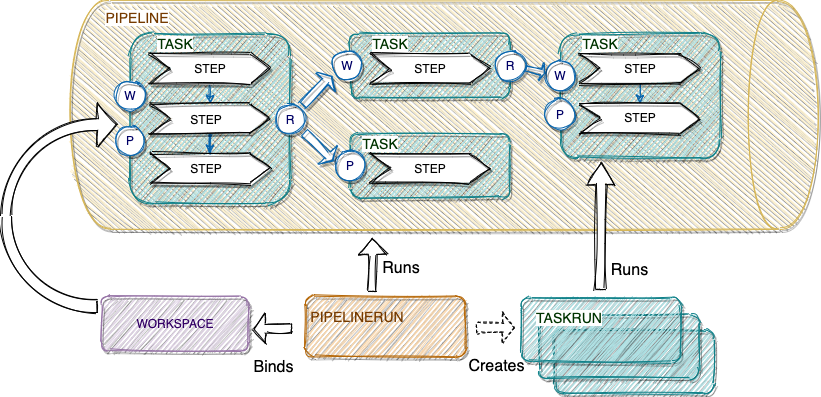
\includegraphics[width=0.5\paperwidth]{img/tekton-workspaces.png}
  \end{textblock*}
  % Knative, Tekton and the CDF
\end{lgrayrwhiteframe}

\section[Authoring]{Authoring}

\begin{sectionwithpicrx}[pierre-bamin--ltjzTfhpCI-unsplash.jpg]{Photo by \href{https://unsplash.com/@bamin}{\underline{Pierre Bamin}}, CC0}
\end{sectionwithpicrx}

\begin{grayframe}
  \frametitle{Steps, Tasks and Teams}
  \begin{itemize}
    \item units of reuse
    \item Steps for small scripts of OTS images
    \item we don't want large shell scripts embedded in YAML
    \item Tasks == pods, cheap I/O
    \item Tasks do one thing well, stable interface
    \item Tasks are re-usable, produced by "experts"
  \end{itemize}
  % units of reuse
  % Steps for small scripts of OTS images
  % we don't want large shell scripts embedded in YAML
  % Tasks == pods, cheap I/O
  % Tasks do one thing well, stable interface
  % Tasks are re-usable, produced by experts
\end{grayframe}

\begin{grayframe}
  \frametitle{Catalog and Hub}
  \begin{itemize}
    \item Sharing Tasks and discovery
    \item Hub and API
    \item Tekton Bundles
  \end{itemize}
  % Sharing Tasks and discovery
  % Tekton Bundles
\end{grayframe}

\begin{grayframe}
  \frametitle{The Pipeline}
  \begin{itemize}
    \item Ever growing pipeline
    \item Multiple teams add to it
  \end{itemize}
  % Ever growing pipeline, multiple teams add to it
\end{grayframe}

\section[Running]{Running}

\begin{sectionwithpic}[pexels-ray-bilcliff-1509237.jpg]{Photo by \href{https://www.pexels.com/@raybilcliff}{\underline{Ray Bilcliff}}, CC0}
\end{sectionwithpic}


\begin{grayframe}
  \frametitle{Pipelines \& Triggers}
  \begin{itemize}
    \item Intro to triggers
    \item Running pipelines through triggers
  \end{itemize}
  % Running pipelines and triggers
\end{grayframe}

\begin{grayframe}
  \frametitle{Events}
  \begin{itemize}
    \item Receiving and sending events
    \item Further spread responsibility, break the pipeline
    \item Interop and event SIG
  \end{itemize}
  % Receiving and sending events
  % Further spread responsibility, break the pipeline
  % Interop and event SIG
\end{grayframe}

\section[Bottlenecks]{Bottlenecks}
\begin{sectionwithpicrx}[dan-cristian-padure-LDMgqr8z7ZE-unsplash.jpg]{Photo by \href{https://unsplash.com/@dancristianp}{\underline{Dan-Cristian Pădureț}}, CC0}
\end{sectionwithpicrx}

{
\begin{tblackbgrayframe}{Growing pipelines}
  %\frametitle{Growing pipelines}
  \begin{itemize}
    \item Directed Acyclic Graphs
    \item Large Pipelines (100 nodes, densely connected)
    \item Scale Issues?
  \end{itemize}
  \begin{itemize}
    \item DAG build on every reconcile
    \item Suboptimal code in the DAG computation
    \item Hundreds of nodes and connections
  \end{itemize}
  \begin{textblock*}{0.42\paperwidth}(0.55\paperwidth,0.35\paperheight)
    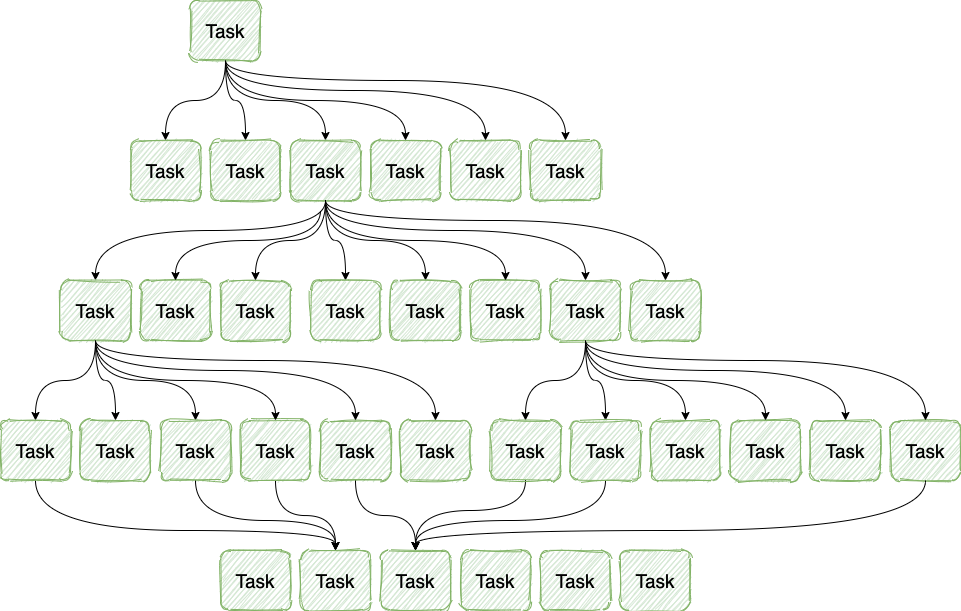
\includegraphics[width=0.42\paperwidth]{img/tekton-large-dag.png}
  \end{textblock*}
\end{tblackbgrayframe}
}

\begin{2columnsframe}%
  {%
    Under Pressure%
  }%
  {%
  Concurrent execution
  \begin{itemize}
    \item Cluster Resources: K8s scheduler
    \item K8s API: Informers
    \item Tekton Controllers: LeaderElection
  \end{itemize}
  \vspace{0.17\textheight}
  Potential enhancements:
  \begin{itemize}
    \item Throttling pipeline execution
    \item Tekton custom scheduler
  \end{itemize}
  }%
  {%
  In real life
  \begin{itemize}
    \item Thousands Tasks/month upstream
    \item Millions containers/month @IBM
    \item Throttling (for security too)
    \item Cluster pollution
  \end{itemize}
  \vspace{0.1\textheight}
  Upcoming features:
  \begin{itemize}
    \item Tekton Results
    \item Performance testing
    \item Metric improvements
  \end{itemize}
  % Many pipelines in parallel / bursts
  % -> Informers, LeaderElection
  % Large execution history
  }
\end{2columnsframe}

\begin{3squares}%
  {%
    Data and I/O
  }%
  {%
  Reusability vs. Efficiency
  \begin{itemize}
    \item Task == Pod % pod creation overhead
    \item Common tasks:
    \begin{itemize}
      \item Clone a git repository
      \item Build a container image
      \item Download content from storage
      \item Run tests
    \end{itemize}
  \end{itemize}
  }%
  {%
  \begin{itemize}
    \item Pods scheduled independently
    \begin{itemize}
      \item Shared storage required (PVC)
      % provisioning time, different features with
      % different back-ends
      \item Extra I/O
      \item Extra execution time
      \item Multi-region clusters
    \end{itemize}
  \end{itemize}
  }%
  {%
  Data in Pipelines
  \begin{itemize}
  \item Metadata: "Results"
  \item Large data: workspace
  \item Alternatives:
    \begin{itemize}
      \item Multiple Tasks in a Pod
      % See pipeline in pipeline, custom tasks
      % Scheduling becomes challenging -> custom scheduler
      \item Re-usable Steps
      % Changes the unit of re-use
      % More complex syntax
      \item Custom scheduler
      % Implementation and maintenance cost
      % Complex problem scape
    \end{itemize}
  \end{itemize}
  }%
  % Unit of re-use and data
  % -> tasks vs pipelines, pod overhead, data across nodes
\end{3squares}

\section[Q\&A]{Thank You! \\Questions?}

\begin{sectionwithpiclargecentral}[carl-jorgensen-5nrnxx_tWe8-unsplash.jpg]{Brecon Beacons, Walse, Photo by \href{https://unsplash.com/@scamartist}{\underline{Carl Jorgensen}}, CC0}
\end{sectionwithpiclargecentral}

\begin{blackframe}
  \frametitle{References}
  \begin{itemize}
    \item \large Come and Join Us at Tekton!
    \item \normalsize Tekton community: \href{https://github.com/tektoncd/community}{github.com/tektoncd/community} \\
  \end{itemize}
  \begin{itemize}
    \item Slides: \href{https://github.com/afrittoli/scaling_pipelines_with_tekton/blob/scd2021/scaling_pipelines_with_tekton.pdf}{github.com/afrittoli/scaling\_pipelines\_with\_tekton}
    \item Tekton: \href{https://tekton.dev}{tekton.dev}
    \item Tekton on GitHub: \href{https://github.com/tektoncd}{github.com/tektoncd}
    \item Performance TEP: \href{https://github.com/tektoncd/community/blob/master/teps/0036-start-measuring-tekton-pipelines-performance.md}{TEP-0036}
    \item Metrics TEP: \href{https://github.com/tektoncd/community/blob/master/teps/0006-tekton-metrics.md}{TEP-0006}
    \item Tekton Results: \href{https://github.com/tektoncd/results}{github.com/tektoncd/results}
  \end{itemize}
  \begin{textblock*}{0.13\paperwidth}(0.73\paperwidth,0.65\paperheight)
    \includesvg[width=0.13\paperwidth]{img/tekton-icon-white.svg}
  \end{textblock*}
\end{blackframe}

\end{document}
